% !TeX spellcheck = en_US
%\documentclass{beamer}
\documentclass[handout]{beamer}
\usepackage[english]{babel}
\usepackage[utf8]{inputenc}
\usepackage{graphicx}
\usepackage{amsmath}
\usepackage{tikz}
\usepackage{multirow}
\usepackage[normalem]{ulem}
\usepackage{subcaption}
%\usepackage{tcolorbox}
\usefonttheme{structuresmallcapsserif}
\usetheme{Antibes}
\usepackage{makecell}

\usecolortheme{whale}
\setbeamertemplate{footline}[frame number]

\usepackage[backend = bibtex, style = verbose, sorting = none, autocite = footnote]{biblatex}
\renewcommand*{\bibfont}{\scriptsize}
\addbibresource{../Documento/bibliography.bib}

%\usepackage[table, dvipsnames]{xcolor}

\newcommand{\sm}[0]{$M_\odot$}
\newcommand{\erf}[1]{\text{erf}\left(#1\right)}
\def\checkmark{{\color{red}\tikz\fill[scale=0.4](0,.35) -- (.25,0) -- (1,.7) -- (.25,.15) -- cycle;}}

\newcommand\blfootnote[1]
{%
	\begingroup
	\renewcommand\thefootnote{}\footnote{#1}%
	\addtocounter{footnote}{-1}%
	\endgroup
}
\newcommand{\fcite}[1]{\blfootnote{\tiny\cite{#1}}}

\expandafter\def\expandafter\insertshorttitle\expandafter{%
	\insertshorttitle\hfill%
	\insertframenumber\,/\,\inserttotalframenumber}

\setbeamerfont{bibliography item}{size=\footnotesize}
\setbeamerfont{bibliography entry author}{size=\footnotesize}
\setbeamerfont{bibliography entry title}{size=\footnotesize}
\setbeamerfont{bibliography entry location}{size=\footnotesize}
\setbeamerfont{bibliography entry note}{size=\footnotesize}

\begin{document}
\begin{frame}
	\centering
%	\color{white}
	\textsc{\LARGE Orbits of black holes in galactic triaxial potentials}
	\\
	\vspace{2.5cm}
	Juan Barbosa\\
	\vspace{1cm}
	\small
	Jaime Forero\\ 
	Advisor\\
	\vspace{0.5cm}
	\footnotesize
	Departamento de F\'isica\\
	Facultad de Ciencias\\
	Universidad de los Andes
\end{frame}

\begin{frame}{Overview}
	\tableofcontents
\end{frame}

\begin{frame}
	\centering
	\Huge
	\scshape
	Introduction
\end{frame}

\section{Introduction}
\begin{frame}{Introduction}
	\begin{columns}
		\begin{column}{0.5\textwidth}
			\begin{figure}[h]
				\centering
				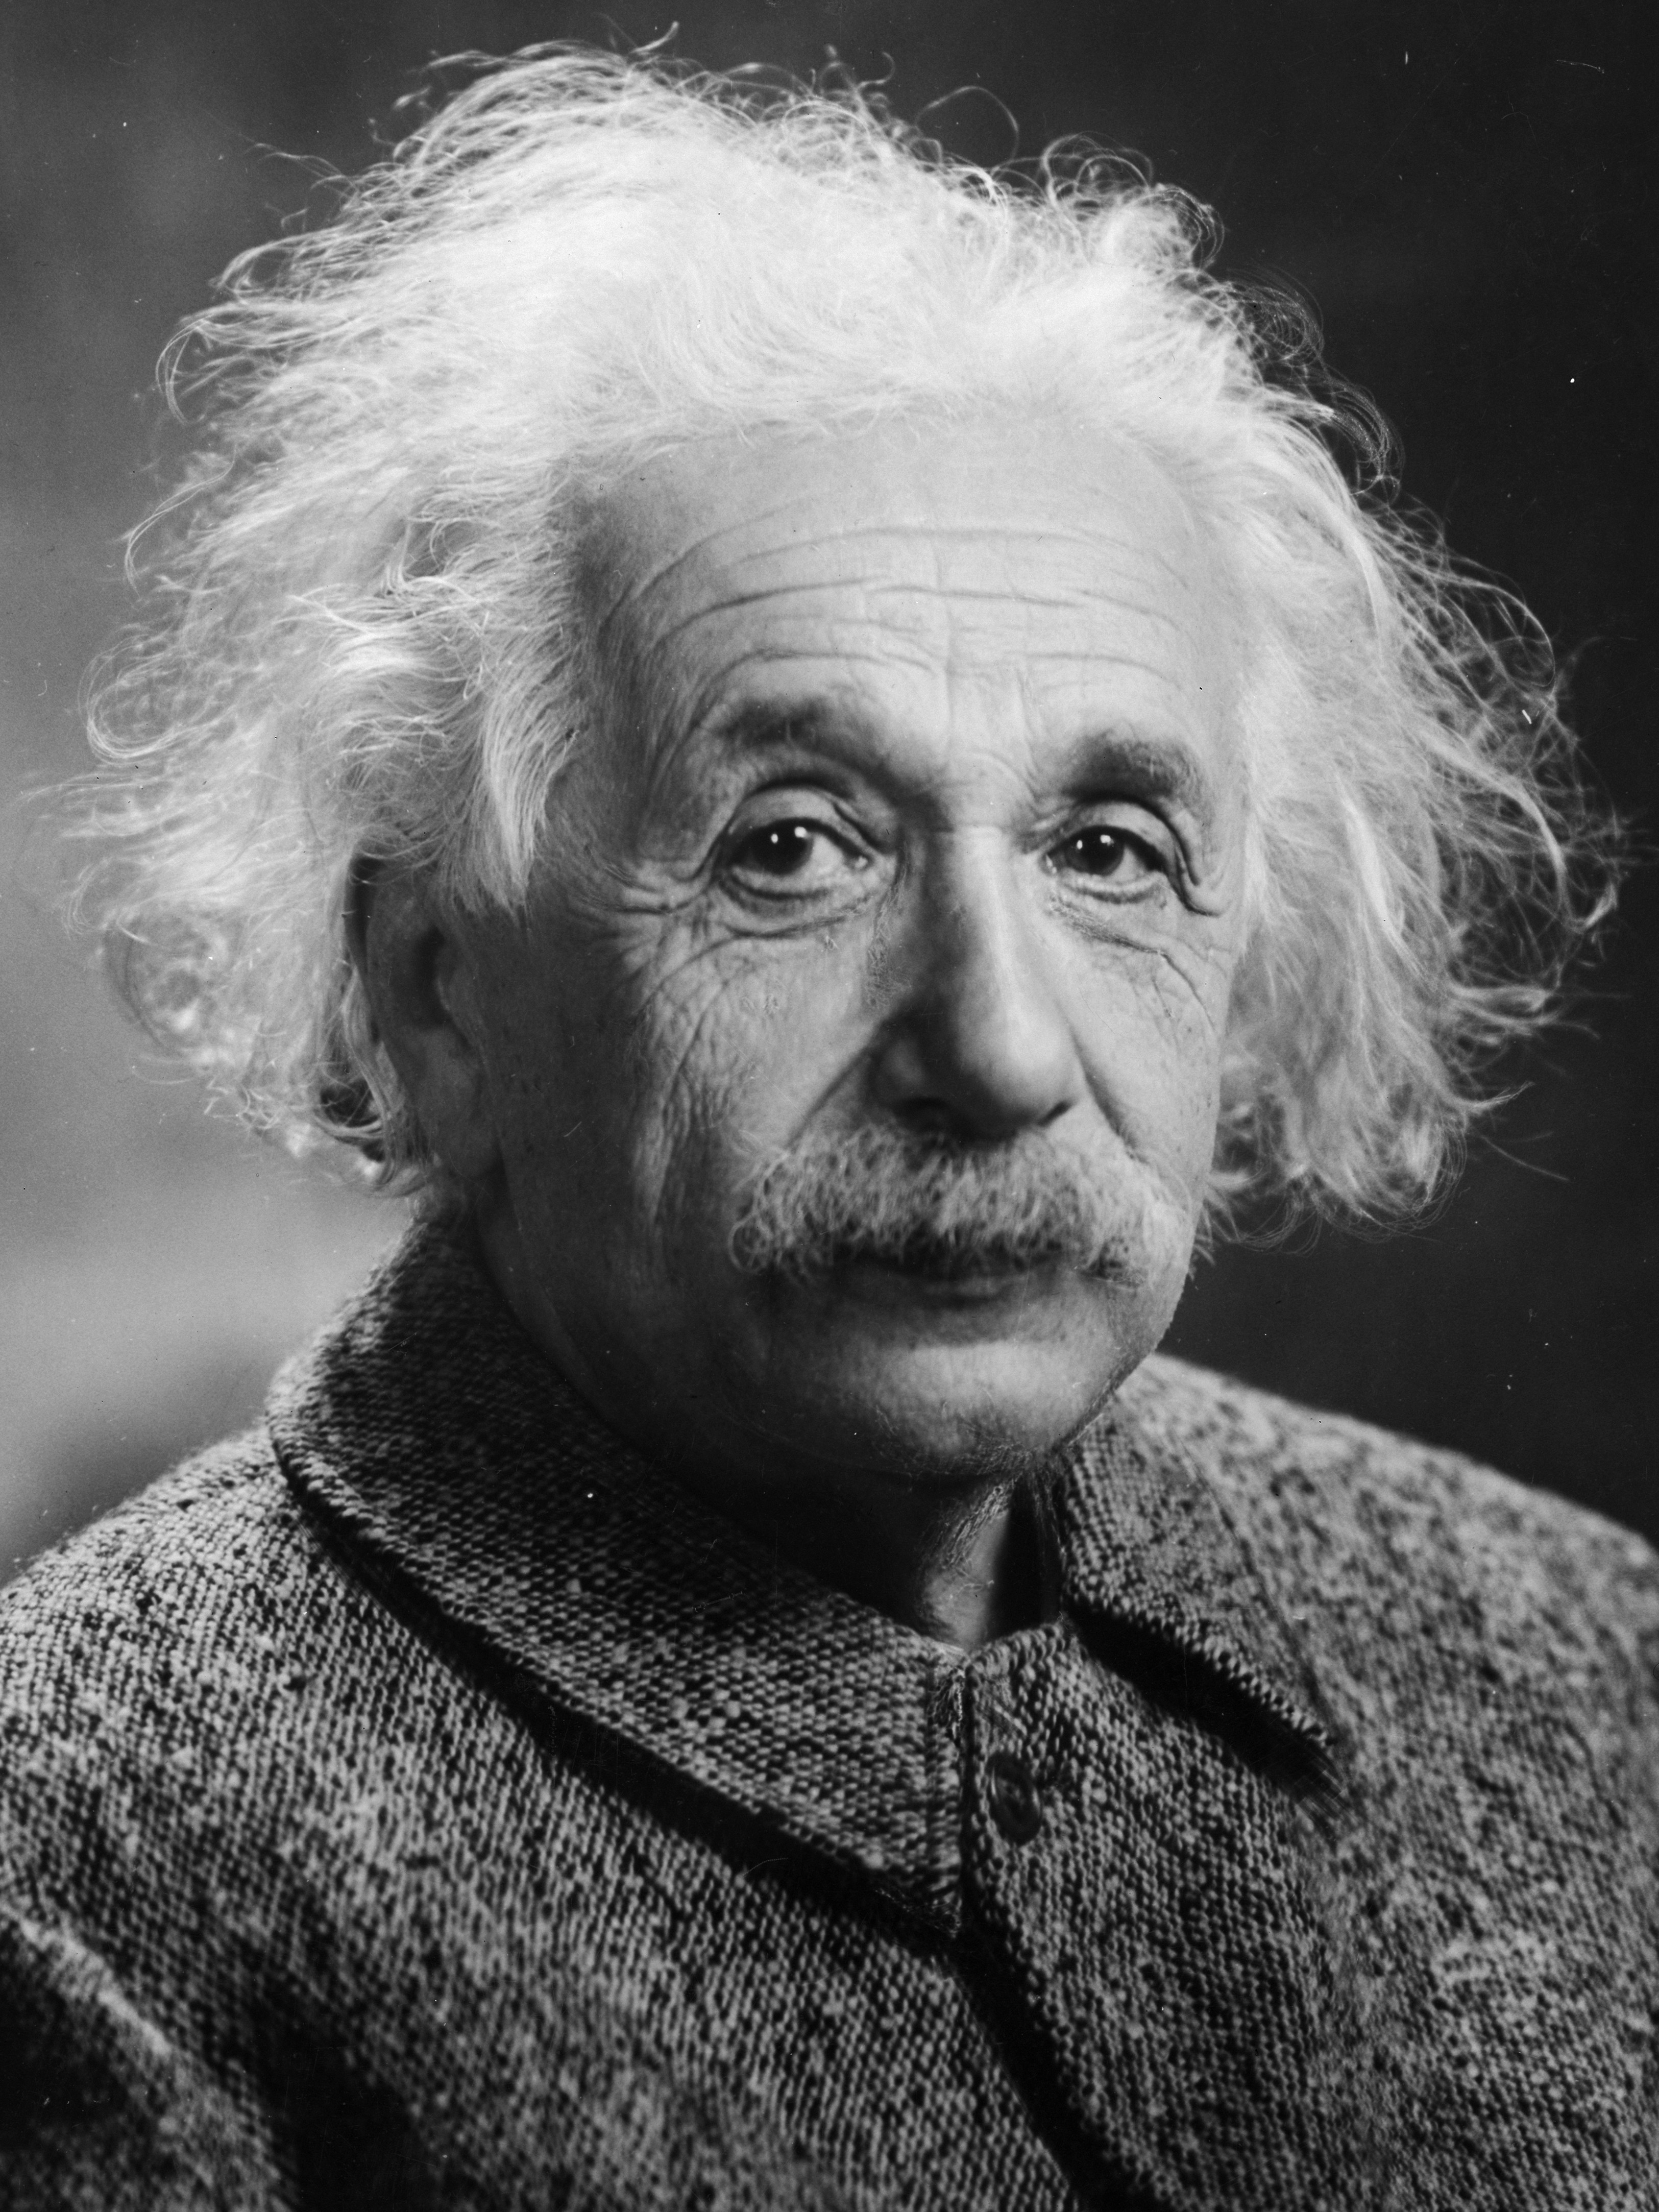
\includegraphics[width=0.9\linewidth]{images/Albert_Einstein_Head}
			\end{figure}
		\end{column}
		\begin{column}{0.5\textwidth}
			\begin{itemize}
				\item Theory of General Relativity, 1916
				\item More than 100 years have passed since the publication of the theory
				\item Today there are gaps in the understanding and implications of Einstein's equations
			\end{itemize}
		\end{column}
	\end{columns}
\end{frame}

\begin{frame}{Introduction}
	\begin{figure}
		\centering
		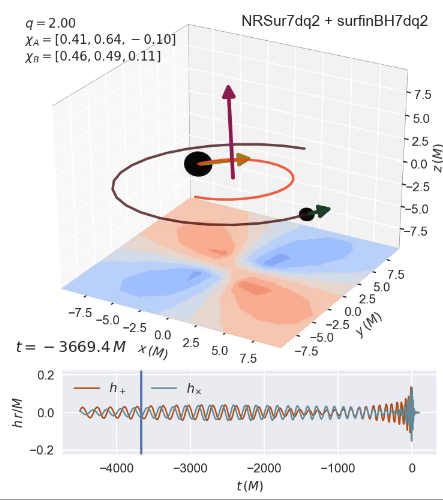
\includegraphics[width=0.4\linewidth]{images/example}
		\caption{\href{run:/home/juan/Documents/TesisFisica/Slides/images/super_kick.mp4}{Binary black hole merger simulation}}
	\end{figure}
	
	\fcite{varma2018binary}
\end{frame}

\begin{frame}{Objectives}
	Study the effect of different triaxial potentials, and initial velocities, on the times required by black holes to return to their initial position, after experiencing a recoil, as well as to quantify how chaotic its trajectory is
	
	\begin{itemize}
		\item Obtain probability distributions for the return properties of the black holes, based on the magnitude and direction of the initial velocity
		\item Study the chaotic behavior of orbits using Lyapunov exponents
%		\item Evaluate the performance of the LeapFrog scheme, used for the numerical integration
	\end{itemize}
\end{frame}

\section{Methodology}
\begin{frame}
	\centering
	\Huge
	\scshape
	Methodology
\end{frame}

\subsection{Galatic setup}
\begin{frame}{Galactic setup}
	\begin{figure}[h]
		\centering
		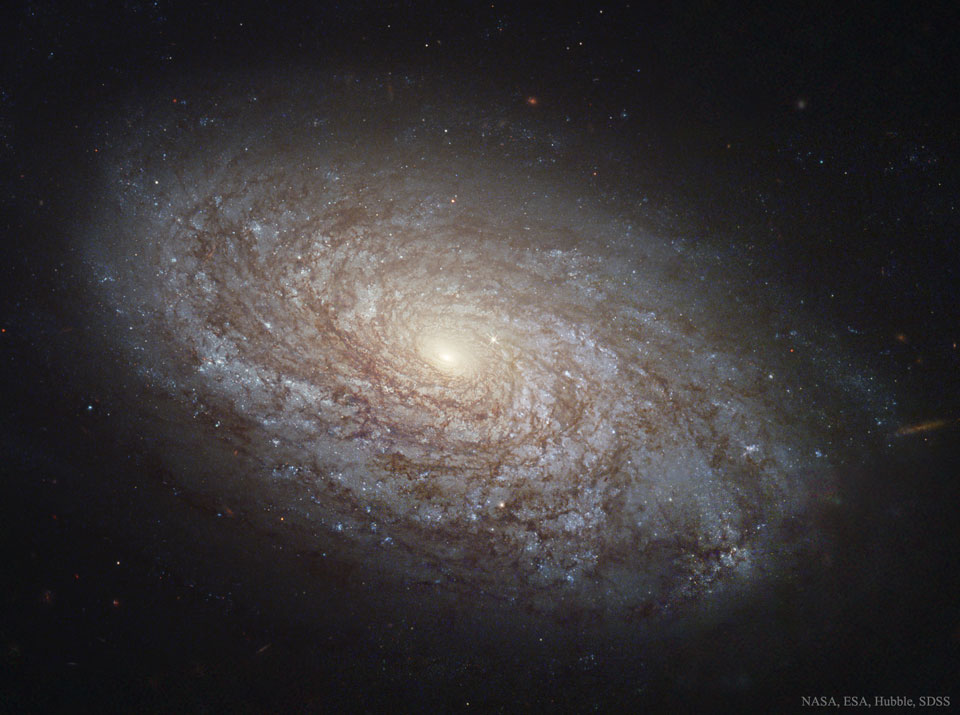
\includegraphics[width=0.8\linewidth]{../Documento/Figures/NGC4414_modified}
		\caption{NGC4414 galaxy as seen by the Hubble telescope.}
	\end{figure}
\end{frame}

%
%\begin{frame}
%	\begin{enumerate}
%		\begin{columns}
%			\begin{column}{0.45\textwidth}
%				\item Gas density (Power law)
%				\begin{figure}[h]
%					\centering
%					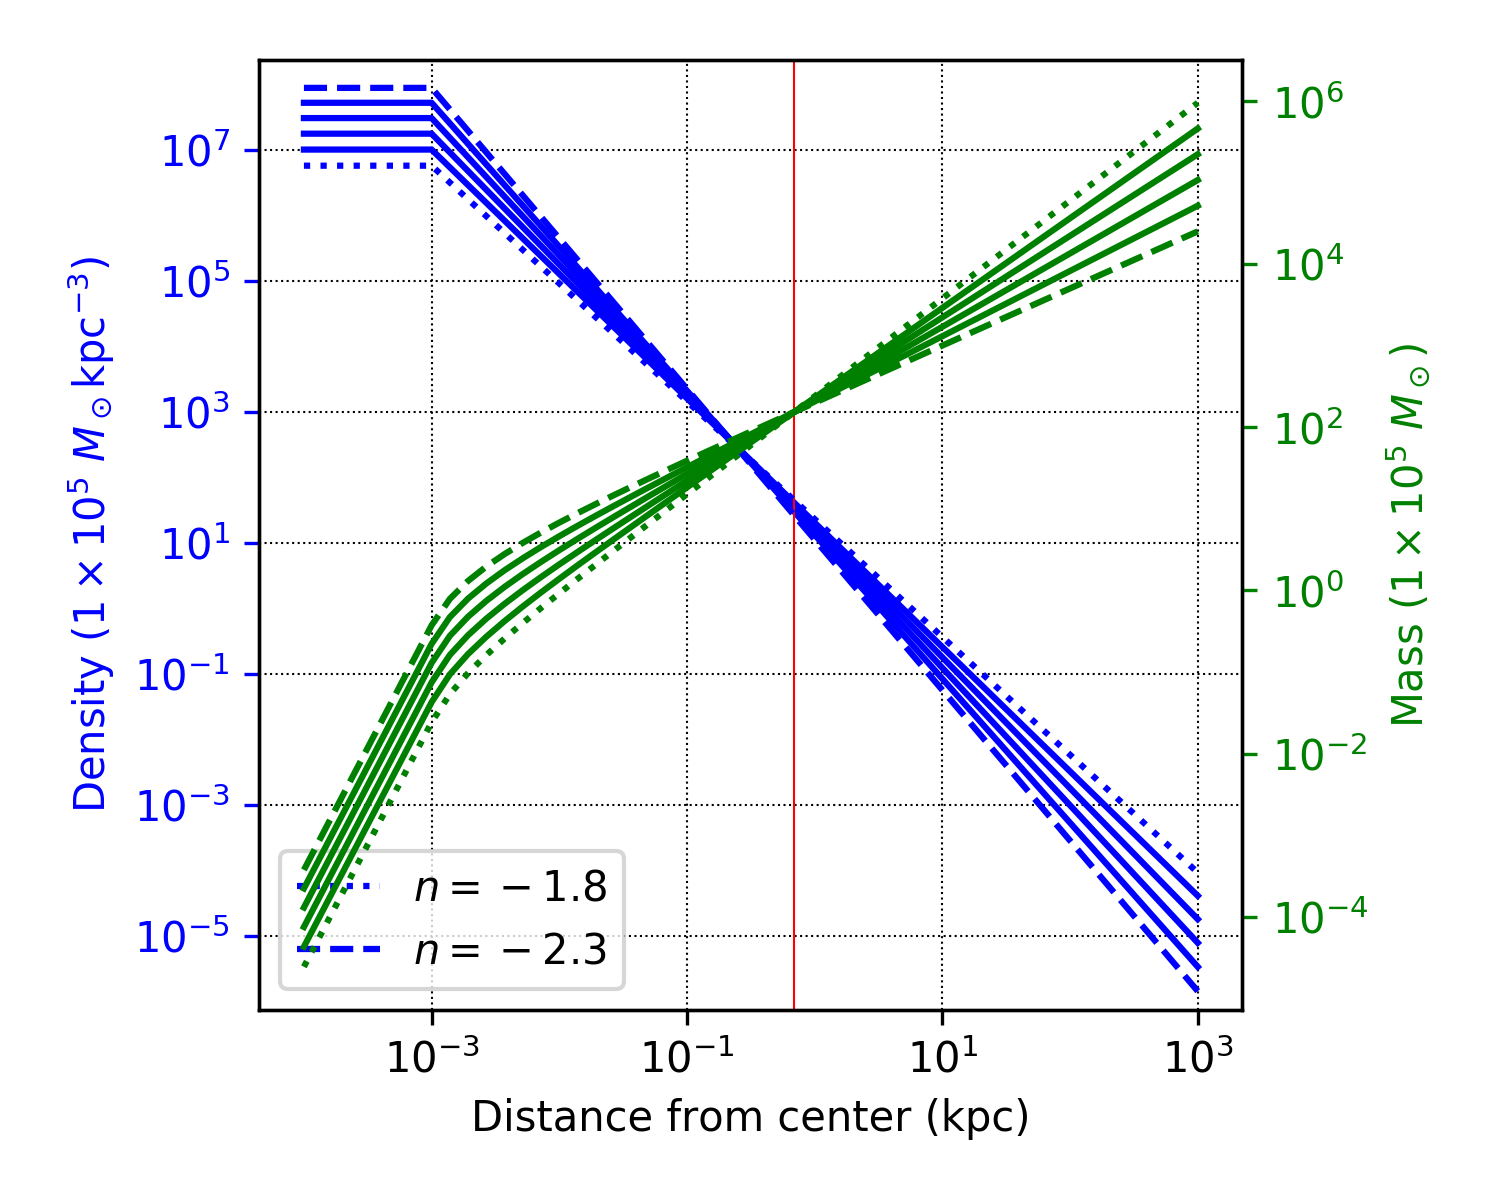
\includegraphics[width=\linewidth]{images/power_law_density_old}
%				\end{figure}
%			\end{column}
%		
%			\begin{column}{0.45\textwidth}
%				\item Gas density (Double power law)
%				\begin{figure}[h]
%					\centering
%					\includegraphics[width=\linewidth]{"../Files/Week 6/power_law_density"}
%				\end{figure}
%			\end{column}
%		\end{columns}
%	\end{enumerate}
%\end{frame}

\begin{frame}{Mass distributions}
	\begin{enumerate}
		\item Dark matter (NWF):
		\begin{equation}\label{eq: dmdensity}
		\rho_\text{DM}(r) = \dfrac{\rho_0^\text{DM}}{\frac{r}{R_s}\left(1 + \frac{r}{R_s}\right)^2}
		\end{equation}
		\item Stellar density (Hernquist):
		\begin{equation}
		\rho_s(r) = \dfrac{f_sf_bM_T \mathcal{R}_s}{2\pi r(r + \mathcal{R}_s)^3}
		\end{equation}
		\item Gas density (Dobule power law):
		\begin{equation}\label{eq: rdensity}
		\rho_\text{gas}(r) = \dfrac{\rho_0^\text{gas}}{\left(1 + \dfrac{r}{r_0}\right)^n}
		\end{equation}
	\end{enumerate}
\end{frame}

%\subsection{Units}
%\begin{frame}{}
%	\begin{table}[h]
%		\centering
%		\caption{Units of measure used on the simulations.}
%		\label{tb: units}
%		\begin{tabular}{c|c}
%			\hline
%			\textbf{Physical property} & \textbf{unit} \\
%			\hline
%			Length & 1 kilo-parsec (kpc) \\
%			Mass & $10^5$ solar masses ($10^5$ \sm) \\
%			Time & 1 giga-year (Gyr) \\
%			\hline
%		\end{tabular}
%	\end{table}
%	\begin{enumerate}
%		\item Universal gravitational constant:
%		\begin{equation}
%			G = 0.4493 \quad \dfrac{\text{kpc$^3$}}{\text{Gy$r^210^5$\sm}}
%		\end{equation}
%		\item Hubble parameter:
%			\begin{equation}
%			H \approx 1.023 H_0 \times10^{-3} \text{ Gyr$^{-1}$} = 6.916\times10^{-2}\text{ Gyr$^{-1}$}
%			\end{equation}
%	\end{enumerate}
%\end{frame}


\subsection{Equation of motion}
\begin{frame}{Equation of motion}
	Trajectories of the kicked black holes are obtained by numerically solving the equation of motion.
	\begin{equation}\label{eq: equationMotion}
		\ddot{\vec{x}} = -a_\text{grav}(\vec{x})\hat{x} + \left(a_\text{DF}(\vec{x}, \dot{\vec{x}})-\dot{x}\dfrac{\dot{M_\bullet}(x, \dot{x})}{M_\bullet}\right)\dot{\hat{x}} 
	\end{equation}
	
	where $M_\bullet$ is the black hole mass
	
	\begin{itemize}
		\item Dark matter, stars and gaseous materials from the medium interact with the black hole adding a drag force
		\item The black hole accretes matter from the surroundings
	\end{itemize}
\end{frame}

\section{Results}
\begin{frame}
	\centering
	\Huge
	\scshape
	Results
\end{frame}

\subsection{Spherical potentials}
\begin{frame}{Spherical potentials}
	\begin{columns}
		\begin{column}{0.4\textwidth}
			\begin{figure}[h]
				\centering
				\includegraphics[width=\linewidth]{"../Files/Week 5/baryonic_fraction_comparison_slides"}
%				\caption{5 \% increase on baryonic fraction decreases return times}
			\end{figure}
			\begin{figure}[h]
				\centering
				\includegraphics[width = 0.9\linewidth]{"../Files/Week 6/power_law_slides"}
%				\caption{Smaller exponents increase the return time}
			\end{figure}
		\end{column}
		\begin{column}{0.7\textwidth}
			$\longleftarrow$ Baryonic fraction
			
			\hspace{2cm} $\bullet$ Stellar fraction
			\begin{figure}[h]
				\centering
				\includegraphics[width=0.9\linewidth]{"../Files/Week 10/returntimes_speed_slides"}
				\caption{Return time for different initial speeds}
			\end{figure}
		
			$\longleftarrow$ Power law exponent
		\end{column}
	\end{columns}	
\end{frame}

\begin{frame}{Effect of the stellar fraction}
	\small
	\begin{equation}\label{eq: fitTr}
	\log_{10}(T_\text{return}) = [a(f_s) v + b(f_s)] + \dfrac{c(f_s)}{v - 1.3}
	\end{equation}
	\begin{table}[h]
		\centering
		\begin{tabular}{lcc}
			\includegraphics[width = 0.3\textwidth]{"../Files/Week 10/a_slides"} & 
			\includegraphics[width = 0.33\textwidth]{"../Files/Week 10/b_slides"} & 
			\includegraphics[width = 0.33\textwidth]{"../Files/Week 10/c_slides"}
		\end{tabular}
	\end{table}
	\small
	\begin{equation}
		a(f_s) = 232f_s^2 + 25 f_s + 2.83
	\end{equation} 
	\begin{equation}
		b(f_s) = -40.7 f_s - 0.75
	\end{equation}
	\begin{equation}
		c(f_s) = 60 f_s^2 - 2.8 f_s - 0.080
	\end{equation}
\end{frame}

\begin{frame}{Effect of the stellar fraction}
	\begin{figure}[h]
		\centering
		\includegraphics[width=0.8\linewidth]{"../Files/Week 10/surface"}
		\caption{Generated surface with the proposed fitting curve}
	\end{figure}
\end{frame}

\subsection{Triaxial potentials}
\begin{frame}{Initial conditions}
	\begin{figure}[h]
		\centering
		\begin{subfigure}[b]{0.475\textwidth}
			\includegraphics[width = \textwidth]{"../Files/Week 13/3d_initial_speeds"}
			\caption{Cartesian}
		\end{subfigure}
		~ 
		\begin{subfigure}[b]{0.475\textwidth}
			\includegraphics[width=\textwidth]{"../Files/Week 13/polar_initial_speeds_slides"}
			\caption{Polar}
		\end{subfigure}
		\caption{Distributions of initial speeds for the triaxial lunches. $\theta$ describes the polar angle and $\phi$ the azimuth.}
		\label{fig: initialSpeedDistributions}
	\end{figure}
\end{frame}

\begin{frame}{Triaxial: Initial conditions}
	\begin{figure}[h]
		\centering
		\includegraphics[width = 0.9\linewidth]{"../Files/Week 13/triaxial_axes"}
		\caption{Distribution of the 28 pair of values for the $y$ and $z$ semiaxis.}
		\label{fig: semiaxisDist}
	\end{figure}
\end{frame}

\begin{frame}{Results}
	\begin{figure}[h]
		\centering
		\includegraphics[width=\linewidth]{"../Files/Week 14/dist_masses"}
		\caption{Mass distributions of the returned black holes}
		\label{fig: massDist}
	\end{figure}
\end{frame}

\begin{frame}{ULAS J1342+0928}
	\begin{columns}
		\begin{column}{0.4\linewidth}
			\begin{figure}[h]
				\centering
				\includegraphics[width=0.8\linewidth]{"images/ULAS"}
				\caption{ULAS J1342+0928 representation}			
			\end{figure}
			\begin{itemize}
				\item Most distant and oldest known SMBH
				\item $Z = 7.54$
				\item $M = 8\times10^8$ $M_\odot$
			\end{itemize}
		\end{column}
		\begin{column}{0.6\linewidth}
			\begin{equation*}\scriptsize
				\begin{array}{ccc}
					Z = 7.54 & \qquad & Z = 20.00 \\
					\downarrow & \Lambda-\text{CDM} & \downarrow \\
					692 \text{Myr} & - & 180 \text{Myr} \\
					\hline
					& 512 \text{Myr} &
				\end{array}
			\end{equation*}
			\begin{figure}
				\centering
				\includegraphics[width=0.95\linewidth]{"../Files/Week 14/masses_at_slides"}
				\caption{Mass distribution at 512 Myr}
				\label{fig: massDistAt}
			\end{figure}
		\end{column}
	\end{columns}
	
\end{frame}

\begin{frame}{Return times}
	\begin{figure}[h]
		\centering
		\includegraphics[width = 0.6\linewidth]{"../Files/Week 14/dist_times_slides"}
		\caption{Return time distributions}
		\label{fig: timeDist}
	\end{figure}
\end{frame}

\begin{frame}{Results}
	\begin{figure}[h]
		\centering
		\begin{subfigure}[b]{0.35\linewidth}
			\includegraphics[width = \linewidth]{"../Files/Week 14/relative_times_slides"}
		\end{subfigure}
		~ 
		\begin{subfigure}[b]{0.35\linewidth}
			\includegraphics[width = \linewidth]{"../Files/Week 14/relative_mass_slides"}
		\end{subfigure}
		\caption{Distributions of the relative return properties.}
		\label{fig: relatives}
	\end{figure}
\end{frame}

\begin{frame}{Results}
	\begin{figure}[h]
		\centering
		\includegraphics[width = 0.7\linewidth]{"../Files/Week 14/lyapunov_orbits"}
		\caption{Orbits with a difference in the initial conditions of 1.9 \%.}
		\label{fig: lyapunov17}
	\end{figure}
\end{frame}










\begin{frame}{Spherical galaxy}
	\begin{figure}[h]
		\centering
		\begin{subfigure}[t]{0.35\textwidth}
			\includegraphics[width = \textwidth]{"../Files/Week 13/images/10_slides_time"}
			\caption{Return times}
		\end{subfigure}
		~ 
		\begin{subfigure}[t]{0.35\textwidth}
			\includegraphics[width=\textwidth]{"../Files/Week 13/images/10_slides_mass"}
			\caption{Return masses}
		\end{subfigure}
		\begin{subfigure}[t]{0.35\textwidth}
			\includegraphics[width=\textwidth]{"../Files/Week 13/images/10_slides_lyapunov"}
			\caption{Lyapunov exponent}
		\end{subfigure}
		\begin{subfigure}[t]{0.35\textwidth}
			\includegraphics[width=\textwidth]{"../Files/Week 13/images/10_ellipsoid"}
			\caption{Geometry}
		\end{subfigure}
		\caption{Distribution of the different properties for the galaxy with $a_1 = 1$, $a_2 = 9.6\times10^{-1}$, $a_3 = 7.0\times10^{-1}$.}
	\end{figure}
\end{frame}

\begin{frame}{Disc galaxy}
	\begin{figure}[h]
		\centering
		\begin{subfigure}[t]{0.35\textwidth}
			\includegraphics[width = \textwidth]{"../Files/Week 13/images/3_slides_time"}
			\caption{Return times}
		\end{subfigure}
		~ 
		\begin{subfigure}[t]{0.35\textwidth}
			\includegraphics[width=\textwidth]{"../Files/Week 13/images/3_slides_mass"}
			\caption{Return masses}
		\end{subfigure}
		\begin{subfigure}[t]{0.35\textwidth}
			\includegraphics[width=\textwidth]{"../Files/Week 13/images/3_slides_lyapunov"}
			\caption{Lyapunov exponent}
		\end{subfigure}
		\begin{subfigure}[t]{0.35\textwidth}
			\includegraphics[width=\textwidth]{"../Files/Week 13/images/3_ellipsoid"}
			\caption{Geometry}
		\end{subfigure}
		\caption{Distribution of the different properties for the galaxy with $a_1 = 1$, $a_2 = 6.9\times10^{-1}$, $a_3 = 1.2\times10^{-2}$.}
	\end{figure}
\end{frame}

\begin{frame}{Bar galaxy}
	\begin{figure}[h]
		\centering
		\begin{subfigure}[t]{0.35\textwidth}
			\includegraphics[width = \textwidth]{"../Files/Week 13/images/22_slides_time"}
			\caption{Return times}
		\end{subfigure}
		~ 
		\begin{subfigure}[t]{0.35\textwidth}
			\includegraphics[width=\textwidth]{"../Files/Week 13/images/22_slides_mass"}
			\caption{Return masses}
		\end{subfigure}
		\begin{subfigure}[t]{0.35\textwidth}
			\includegraphics[width=\textwidth]{"../Files/Week 13/images/22_slides_lyapunov"}
			\caption{Lyapunov exponent}
		\end{subfigure}
		\begin{subfigure}[t]{0.35\textwidth}
			\includegraphics[width=\textwidth]{"../Files/Week 13/images/22_ellipsoid"}
			\caption{Geometry}
		\end{subfigure}
		\caption{Distribution of the different properties for the galaxy with $a_1 = 1$, $a_2 = 6.6\times10^{-2}$, $a_3 = 6.1\times10^{-2}$.}
	\end{figure}
\end{frame}

\section{Conclusions}
\begin{frame}
	\centering
	\Huge
	\scshape
	Conclusions
\end{frame}

\begin{frame}{Conclusions}
	\begin{itemize}
		\item Including triaxiality in galaxies can shift the predictions from previous spherical studies
		\begin{itemize}
			\item On average, return times for triaxial studies are 2.6 times longer than those	expected in spherical galaxies
			\item Masses, on the other hand, show an average increase of 24 \%
		\end{itemize}
		\item Person correlation between the return properties (time and mass) has been quantified at 0.63
		\item The probability of finding a black hole such as the ULAS J1342+0928 quasar in the simulations is 0.34 \%
		\item The baryonic fraction of the galaxy, the power law
		exponent of the gas profile, and the amount of stars drastically alter the return properties of a black hole
	\end{itemize}
\end{frame}

\begin{frame}{Conclusions}
	\begin{itemize}
		\item Lyapunov exponents show that there is a proportional dependency with the magnitude of the initial velocity
		\item More chaotic orbits are related with the highest potential axis (major semiaxis)
	\end{itemize}
\end{frame}

\begin{frame}
	\centering
	\Huge
	\scshape
	Thank you
\end{frame}

\section{References}
\begin{frame}{References}
	\nocite{*}
	\printbibliography
\end{frame}

%\begin{frame}{Triaxial setup}
%	Density shells for each profile are ellipsoids
%	\begin{equation}
%	m^2(\vec{x}) \equiv x_1^2 + \left(\dfrac{a_1}{a_2}\right)^2x_2^2 + \left(\dfrac{a_1}{a_3}\right)^2x_3^2
%	\end{equation}
%	
%	A thin shell, whose inner and outer skins are the surfaces $m$ and $m + \delta m$ is described by:
%	\begin{equation}\label{eq: m2}
%	m^2(\vec{x}, \tau) = a_1^2\left(\frac{x_1^{2}}{\tau + a_{1}^{2}} + \frac{x_2^{2}}{\tau + a_{2}^{2}} + \frac{x_3^{2}}{\tau + a_{3}^{2}}\right)
%	\end{equation}
%	where $\tau \geq 0$ labels the surfaces \fcite{binney2011galactic}
%\end{frame}
%
%
%\begin{frame}
%	\begin{columns}
%		\begin{column}{0.3\linewidth}
%			\begin{figure}[h]
%				\centering
%				\includegraphics[width = \linewidth]{"../Files/Week 7/triaxial_mass_issue"}
%				\caption{Effective gravitational mass}
%				\label{fig: triaxial_mass_issue}
%			\end{figure}
%		\end{column}
%		\begin{column}{0.7\linewidth}
%			The contributions of all ellipsoidal shells that make up the profile are taken into account
%			\begin{equation}
%				\psi(m) \equiv \int\limits_{0}^{m^2} \rho(m^2)dm^2 = \int\limits_{0}^{k = m^2} \rho(k)dk
%			\end{equation}
%			
%			The potential of any body in which $\rho = \rho(m^2)$ is:
%		\end{column}
%	\end{columns}
%	\begin{equation}\label{eq: generalPotential}
%	\Phi(\vec{x}) = -\pi G \dfrac{a_2a_3}{a_1}\int\limits_{0}^{\infty}\dfrac{\psi(\infty) - \psi(m)}{\sqrt{(\tau + a_1^2)(\tau + a_2^2)(\tau + a_3^2)}}d\tau
%	\end{equation}
%	\fcite{binney2011galactic}
%\end{frame}
%
%\begin{frame}
%	Numerical integration of the gradients of the potentials is made with Simpson 3/8 rule.
%	\begin{equation}
%		\nabla \Phi_\text{DM}(\vec{x}) = 2 \pi G R_{s}^{3}\rho_0 a_{1} a_{2} a_{3} \displaystyle\int\limits_{0}^{\infty}
%		\dfrac{\vec{\phi}(\vec{x}, \tau) d\tau}{m(\vec{x}, \tau)\left(R_{s} + m(\vec{x}, \tau)\right)^{2}}	
%	\end{equation}
%	\begin{equation}
%		\nabla \Phi_\text{S}(\vec{x})= G M_{s} a_{1} a_{2} a_{3} \displaystyle\int\limits_{0}^{\infty} \frac{ \vec{\phi}(\vec{x}, \tau) d\tau}{m(\vec{x}, \tau)\left(\mathcal{R_s} + m(\vec{x}, \tau)\right)^{3}}
%	\end{equation}
%	
%	\begin{equation}
%		\small
%		\nabla \Phi_\text{G}(\vec{x}) = 2 \pi G \rho_0 a_{1} a_{2} a_{3}
%		\left\{
%		\begin{array}{l}
%		\displaystyle\int\limits_{0}^{\infty} \vec{\phi}(\vec{x}, \tau) d\tau \qquad \text{for $m(\vec{x}, \tau) < r_0$}\\
%		r_{0}^{- n} \displaystyle\int\limits_{0}^{\infty} m(\vec{x}, \tau)^{n}  \vec{\phi}(\vec{x}, \tau) d\tau \qquad \text{else}
%		\end{array}
%		\right.		
%	\end{equation}
%\end{frame}

%\subsubsection{Results}
%\begin{frame}{Triaxial}
%	\begin{figure}[h]
%		\centering
%		\begin{subfigure}[t]{0.45\textwidth}
%			\includegraphics[width = \textwidth]{"../Files/Week 7/symmetric"}
%%			\caption{Spherical case}
%%			\label{fig: symmetricDensity3d}
%		\end{subfigure}
%		~ 
%		\begin{subfigure}[t]{0.45\textwidth}
%			\includegraphics[width=\textwidth]{"../Files/Week 7/triaxial"}
%%			\caption{Triaxial case with ($a_1$:$a_2$:$a_3$) = (1:0.5:0.3)}
%%			\label{fig: triaxialDensity3d}
%		\end{subfigure}
%		\begin{subfigure}[t]{0.6\textwidth}
%			\includegraphics[width=\textwidth]{"../Files/Week 7/ellipsoid_"}
%%			\caption{Equicentred ellipsoids with ($a_1$:$a_2$:$a_3$) = (1:0.5:0.3)}
%		\end{subfigure}
%		\caption{Dark matter densities comparison between spherical and triaxial cases.}
%		\label{fig: symmetricTriaxial}
%	\end{figure}
%\end{frame}

%\begin{frame}
%	\begin{figure}[h]
%		\begin{tabular}{cc}
%			\includegraphics[width = 0.7\textwidth]{"../Files/Week 10/3dorbit"} &
%			\includegraphics[width = 0.3\textwidth]{"../Files/Week 10/3dorbit_distances"}
%		\end{tabular}
%	\end{figure}
%\end{frame}

%
%\begin{frame}{Results}
%	\begin{figure}[h]
%		\centering
%		\begin{tabular}{cc}
%			\includegraphics[width = 0.49\textwidth]{"../Files/Week 7/error"} & 
%			\includegraphics[width = 0.49\textwidth]{"../Files/Week 7/symmetric_triaxial"}
%		\end{tabular}
%		\caption{Differences for analytical and numerical integration of the potentials. Analytical is taken as: $GM(r) / r^2$}
%		\label{fig: numericalErrors}
%	\end{figure}
%\end{frame}

%\begin{frame}
%	\begin{figure}[h]
%		\begin{tabular}{cc}
%			\includegraphics[width = 0.6\textwidth]{"../Files/Week 7/orthogonal_triaxial"} &
%			\includegraphics[width = 0.4\textwidth]{"../Files/Week 7/ellipsoid"}
%		\end{tabular}
%		\caption{Orthogonal launches for a triaxial profile with semi-axis ($a_1$:$a_2$:$a_3$) = (1 : 0.99 : 0.95)}
%		\label{fig: mainOrthogonalLaunches}
%	\end{figure}
%\end{frame}
%
%\begin{frame}{}
%	\begin{figure}[h]
%		\begin{tabular}{cc}
%			\includegraphics[width = 0.6\textwidth]{"../Files/Week 11/lyapunov_distances"} &
%			\includegraphics[width = 0.4\textwidth]{"../Files/Week 11/lyapunov_orbits"}
%		\end{tabular}
%	\end{figure}
%\end{frame}

%\begin{frame}
%	\begin{center}
%		\scshape\huge
%		Thank You
%	\end{center}
%\end{frame}

%
%
%
%
%
%
%
%
%
%
%
%
%
%
%
%
%
%
%
%
%\begin{frame}
%	Computer simulations are sensitive to rounding errors due to the lack of infinite precision when representing decimal numbers.
%	\begin{figure}[h]
%		\centering
%		\includegraphics[width=0.7\linewidth]{"../Files/Week 3/floating"}
%		\caption{Floating point precision for different values, for a 32 bit and 64 bit holders.}
%		\label{fig: IEEE-754}
%	\end{figure}
%\end{frame}
%
%\begin{frame}
%	Mass distributions between components are given by:
%	\begin{equation}
%		M_\text{DM}(R_\text{vir}) = (1 - f_b)M_h
%	\end{equation}
%	\begin{equation}
%		M_\text{stars}(R_\text{vir}) = f_sf_bM_h
%	\end{equation}
%	\begin{equation}
%		M_\text{gas}(R_\text{vir}) = (1 - f_s)f_bM_h
%	\end{equation}
%	
%	with $f_b = 0.156$ and $M_h = 10^8$ \sm
%	\begin{equation}
%		R_\text{vir} = \left({\dfrac{M_hG}{100 H(t)^2}}\right)^{1/3}
%	\end{equation}
%\end{frame}
%
%\begin{frame}{Dynamical friction}
%	As the black hole travels through the galaxy, dark matter, stars and gaseous materials from the medium interact with the black hole adding a drag force.
%	\begin{figure}[h]
%		\centering
%		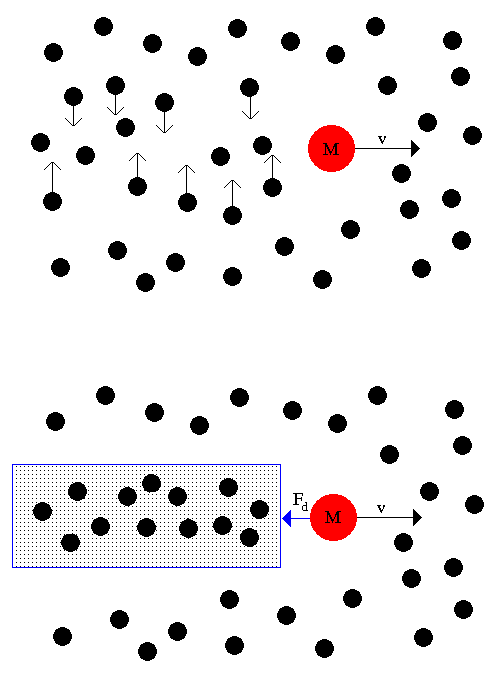
\includegraphics[width = 0.25\linewidth]{images/dyn_friction}
%		\caption{Collisionless dynamical friction}
%	\end{figure}
%	\fcite{df_image}
%\end{frame}
%
%\begin{frame}
%	\begin{itemize}
%	\item Collisionless matter interacts with the black hole gravitational only
%	\begin{equation}\label{eq: df_cl}
%	a_\text{DF}^\text{cl}(\vec{x}, \dot{\vec{x}}) = -\dfrac{4\pi G^2}{\dot{x}^2} M_\bullet\rho(\vec{x})\ln\Lambda\left(\erf{X} - \dfrac{2}{\sqrt{\pi}}Xe^{-X^2}\right)
%	\end{equation}
%	
%	\item On the other side gas is in direct contact with the black hole
%	\begin{equation}\label{eq: df_c}
%	a^\text{c}_\text{DF}(\vec{x}, \dot{\vec{x}}) = -\dfrac{4\pi G^2}{\dot{x}^2}M_\bullet\rho_\text{gas}(\vec{x})f(\mathcal{M})
%	\end{equation}
%	\end{itemize}
%\end{frame}
%
%\begin{frame}{Accretion into the black hole}
%	As the black hole accretes matter from the surroundings, an acceleration appears, due to the second law of Newton.
%	\begin{equation}
%	\dot{M}_\bullet(\vec{x}, \dot{\vec{x}}) = \left\{
%	\begin{array}{lc}
%	\dot{M}_\bullet^\text{BHL}(\vec{x}, \dot{\vec{x}}) & \text{if $\dot{M}_\bullet^\text{BHL} < \dot{M}_\bullet^\text{Edd}$} \\
%	\dot{M}_\bullet^\text{Edd} & \text{else}
%	\end{array}
%	\right.
%	\end{equation}
%	
%	\begin{equation}
%	\dot{M}_\bullet^\text{BHL}(\vec{x}, \dot{\vec{x}}) = \dfrac{4\pi G^2 \rho_G(\vec{x})M^2_\bullet}{\left(c_s^2 + \dot{x}^2\right)^{3/2}} % \qquad \text{with } \rho_B(\vec{x}) = \rho_\text{stars}(\vec{x}) + \rho_\text{gas}(\vec{x})
%	\end{equation}
%	\begin{equation}
%	\dot{M}_\bullet^\text{Edd} = \dfrac{(1 - \epsilon)M_\bullet}{\epsilon t_\text{Edd}} \qquad \epsilon = 0.1, \quad t_\text{Edd} = 0.44 \text{ Gyr}
%	\end{equation}
%\end{frame}
%
%\begin{frame}
%	Drag generated by gas depends on local sound speed
%	\begin{equation}
%		\mathcal{M}(\dot{x}) \equiv \dfrac{|\dot{x}|}{c_s} = |\dot{x}|\sqrt{\dfrac{\mathcal{M}_w}{\gamma RT_\text{vir}}} = |\dot{x}|\sqrt{\dfrac{\mathcal{M}_w}{\gamma R}\left(\dfrac{2k_BR_\text{vir}}{\mu m_p G M_h}\right)}
%	\end{equation}
%	\begin{equation*}
%		\mathcal{M}(\dot{x}) = 1.63|\dot{x}|\sqrt{\dfrac{R_\text{vir}}{M_h}}
%	\end{equation*}
%	
%	\begin{equation}\label{eq: df_c}
%	a^\text{c}_\text{DF}(\vec{x}, \dot{\vec{x}}) = -\dfrac{4\pi G^2}{\dot{x}^2}M_\bullet\rho_\text{gas}(\vec{x})f(\mathcal{M})
%	\end{equation}
%	
%	with
%	\begin{equation}\footnotesize
%	f(\mathcal{M}) = \left\{
%	\begin{matrix}
%	0.5\ln\Lambda \left[\erf{\dfrac{\mathcal{M}}{\sqrt{2}}} - \sqrt{\dfrac{2}{\pi}}\mathcal{M}e^{-\mathcal{M}^2/2}\right]& \text{if $\mathcal{M} \leq 0.8$}\\
%	1.5\ln\Lambda \left[\erf{\dfrac{\mathcal{M}}{\sqrt{2}}} - \sqrt{\dfrac{2}{\pi}}\mathcal{M}e^{-\mathcal{M}^2/2}\right] & \text{if $0.8 < \mathcal{M} \leq \mathcal{M}_{eq}$}\\
%	0.5\ln\left(1 - \mathcal{M}^{-2}\right) + \ln\Lambda & \text{if $\mathcal{M} > \mathcal{M}_{eq}$}
%	\end{matrix}
%	\right.
%	\end{equation}
%\end{frame}
%
%\begin{frame}
%	\begin{equation}
%		\omega = \dfrac{\tau^\gamma}{\tau^\gamma + 1}, \qquad \tau = \left(\frac{\omega}{1-\omega}\right)^{\frac{1}{\gamma}}, \qquad d\tau = \dfrac{\left(- \frac{\omega}{\omega - 1}\right)^{\frac{1}{\gamma}}}{\gamma \omega \left(- \omega + 1\right)}
%	\end{equation}
%	
%	\begin{equation}
%		\phi_i(x_i, \tau) = \dfrac{x_i}{\left(\tau + a_i^2\right)^{\frac{3}{2}} \prod\limits_{i \neq j}^3\sqrt{\tau + a_j^2}}
%	\end{equation}
%	\begin{equation}
%		\vec{\phi}(\vec{x}, \tau) = (\phi_1(x_1, \tau), \phi_2(x_2, \tau), \phi_3(x_3, \tau))
%	\end{equation}
%\end{frame}

\end{document}